\chapter{Questions}
\label{questions-chapter}
% TODO: rewrite to avoid overuse of important.
% TODO: Hey! This is a good idea. I should do it! It's not trivial but
% shouldn't be hard.
% along with
% various kinds of backoff, for example, to bigrams or coarser node
% tags.
The state of syntax measures in dialectometry described above leaves
several research questions unresolved. It is not yet clear whether $R$
is a good measure of syntax distance. Previous results have shown that
it can obtain significant distances, but has either failed to do so
reliably, as in my work on British English \cite{sanders08b}, or has
not compared traditional dialect areas, as in
\namecite{nerbonne06}. $R$, and statistical methods as a whole, still
need to show that they can contribute to dialectometry's study of
syntax.

This leads to the first question: will the features found by
dialectologists agree with the highly ranked features used by $R$ for
classification? I will investigate this question by comparing $R$'s
results to the syntactic dialectology literature on Swedish. A
secondary, but related question is whether the regions of Sweden
accepted by dialectology will be reproduced by $R$. For example, my
previous research on British English reproduced the well-known North
England-South England dialect regions. However, this dissertation
eliminates the corpus variability in that research
\cite{sanders08b}. With a corpus collected collected for the purpose
of dialect research, and with a phonological corpus transcribed from the
same interviews, more precise comparisons should be possible, both
between regions and between syntax and phonology.

Additionally, if $R$ is found to be a bad measure of syntax distance,
this dissertation evaluates a number of alternative
measures, such as Kullbeck-Leibler divergence and cosine
dissimilarity. $R$ is one way to aggregate features that are created
by decomposing sentences. It treats features as atomic, and does not
manipulate them in any syntax-specific ways. As such, $R$ differs from
Goebl's WIV only in being designed for larger feature sets and
larger corpora. Both assume that independent, atomic features derived
from a sentence can adequately capture dialect differences. If this is
not the case, then a more syntax-specific measure will be needed.

A secondary question, relevant once a useful syntax distance measure
is established, is what input features cause $R$ to produce the best
results. Choice of feature set is at least as important as choice of
distance measure. Feature set My previous work on British English showed that
leaf-ancestor paths provide a small advantage over part-of-speech (POS)
trigrams, presumably by capturing syntactic structure higher in the
parse tree. And, whereas development of a statistical distance measure
is difficult, new feature sets can be developed relatively quickly.
% on average, each committee meeting results in 2.1 new feature sets
% being proposed, and only 0.7 new distance measures.
In this dissertation, I evaluate several sets besides POS trigrams and
leaf-ancestor paths, such as phrase structure rules, dependency paths,
and lexical trigrams. I also evaluate variants of these feature sets,
for example varying the POS tagger or POS tag set. I also evaluate
combined feature sets.

Feature sets can be evaluated by comparing performance of different
feature sets on a fixed corpus and with a fixed distance
measure. Here, performance is measured using the same criteria as for
distance measures: the number of significant distances between regions
and the similarity of the results to those found by dialectologists.

A final question is whether the syntactic dialectometry practiced here
agrees with phonological dialectometry on the same corpus. Unlike the
previous questions, which use agreement between syntactic
dialectometry and dialectology, there is no {\it a priori} reason to
expect syntax/phonology agreement; it is quite possible that
phonological features create one set of boundaries while syntactic
feature create another set. However, agreement between the two would
be further evidence for that $R$ succeeds in establishing syntactic
dialectometry.

\section{Question 1 : Agreement with Dialectology}

At a high level, the first question is whether $R$, as a measure from
dialectometry, agrees with dialectology. On closer inspection, this
question covers a number of more specific questions, each dealing with
a specific comparison to dialectology. The first is whether the
features that $R$ counts most important are the same as the features
discussed in the dialectology literature. The other questions are
whether boundaries, regions and distances found by $R$ agree with
dialectology.

Feature agreement is the most important and most difficult
question. It is the most important for two reasons. First, it offers
the most precise explanation and is the easiest to disprove.
% ie easiest to find a counter-example in the literature
Second,
dialectology starts with individual features, so the most work for
comparison is available at the feature level.

\subsection{Dialectology}

Definition of terms from dialectology is appropriate here, along with
an explanation of how they fit together. The basic unit in
dialectology is the feature, which corresponds to a feature given to
$R$. During analysis, the linguist may suspect that a feature is
characteristic of a particular region, but more information, usually
from a survey, is needed to make certain.

Given a survey or other source of geographical mapping information, a
boundary for a feature can be delineated. This boundary is called an
isogloss. With the right information, isoglosses are usually simple to
determine. One complicated case has a few occurrences of a feature
variant stranded in the middle of the other variant. This complicates
the geometry of the isogloss.

If a number of isoglosses coincide, they form an isogloss bundle,
which separates one region from another. Isogloss bundles are simple
in theory, but in practice they are difficult to find because
isoglosses rarely coincide perfectly. In practice, undisputed isogloss
bundles only occur between well-known dialects, such as the
boundaries between Low and High German or Northern and Southern
English of England. In cases where more precision is required, there
is not usually a sufficient number of coincident isoglosses. Even
though there may be plenty of isoglosses in the area, isoglosses so
rarely coincide that only a few may be construed as forming an
isogloss boundary.

Dialectology does not have a clear equivalent to dialectometry's
distance. The closest analog is size of isogloss bundle; to reflect
this, dialect maps typically indicate size of isogloss bundle by
thickness of boundary line. Additionally, some regions are known to differ from
others much more than the rest of the regions. This usually mirrors
isogloss bundles, surfacing in the literature as a list of well-known
dialect features of a region.

\subsection{Features}

To match the features of dialectology to the features that $R$ uses to
produce a distance, I first need to find discussion of Swedish dialect
features in the dialectology literature. For example,
\namecite{rosenkvist07} discusses the South-Swedish apparent
cleft. This feature is best analyzed as a single feature; Rosenkvist
mentions that it occurs in southern and central Swedish and not
northern Swedish, but does not give a more precise location than
``Svealand and G\"otaland''. So we will compare this feature directly
to features found in any part of the corpus.

Next I convert the feature to the formalism used for annotation.
Typically this requires conversion of a minimalist structure to a
simpler structure based on a phrase-structure grammar. This produces a
skeleton parse or parse fragment. Then the skeletal structure can be
broken into features in the same way that parses of corpus sentences
are. Once converted, the feature should appear in the list of
important features for regions in southern Sweden.

In the apparent cleft example, the apparent cleft is realized as an
additional use of the word {\it som}, ordinarily a
complementizer. Typically, the next step is to identify the minimalist
structure for this, but Rosenkvist's 2007 paper does not yet provide
this analysis. Although there is no structure to translate to a
phrase-structure skeleton, his analysis provides enough clues to
produce some features directly. Trigrams are easiest; he mentions that
his corpus search used the strings {\it det \"ar som} (``It is that'')
and {\it det \"ar bara som} ``It's just that''. These words only need
part-of-speech annotation to be trigram features. Dependency
paths can also use these parts of speech for the local dependencies
between {\it det,\"ar} and {\it som}. Rosenkvist also mentions
some syntactic properties of apparent clefts that are useful for
specifying dependency path features: the subject of the {\it
  som}-clause must be a pronoun, so we should expect to see
dependency paths of the form {\it ROOT-som-PRON} in the regions that
have the apparent cleft.

Once dialectometric features have been specified from some linguistic
analysis, the analysis consists of the following questions: in what
regions do these features appear? Do these regions match the expected
distribution (if any) from the linguistic analysis? How much do
the features contribute to distance from other regions? If there are
other features that contribute more, what are they?

% TODO: Finish example by using structure from papers on the apparent
% cleft (if it exists) in English and Japanese.

\subsection{Isogloss Boundaries}
%add connective sentences! or paragraph!

Isogloss boundaries are intermediate in complexity between features unspecified
for location and regions demarcated by isogloss bundles. For the
purposes of this dissertation, however, there is not much difference
between a feature with some documented locations and an isogloss
boundary. An isogloss makes the regions of interest clearer, but it is
a difference in degree and not in quality. The real difference in
analysis occurs when dialectology has identified an isogloss bundle.

\subsection{Isogloss Bundles}
%add connective sentences! or paragraph!

Isogloss bundles compare straightforwardly to dialectometry, insofar as
dialectometric methods produce regions. There are two primary ways for
identifying regions from these methods: hierarchical clustering and
multi-dimensional scaling. Neither method is perfect; as with isogloss
bundles, some human input is still needed to determine whether an
inter-region boundary truly exists at some point.

Hierarchical clustering
produces well-delineated regions, at the cost of some
uncertainty---the results tend to vary quite a bit from feature set to
feature set. Only clusters that persist between results from multiple
feature sets should be considered valid.

In contrast, multi-dimensional scaling (MDS) is a straightforward
mathematical transformation of the high-dimensional space created by
measuring distances between all regions in the corpus. Although MDS
does not produce spurious information, its results are often hard to
analyze because it produces boundaries of varying strength. Very
different regions stand out, but similar regions appear similar even
if they contain some differences. This similarity can make it
difficult to decide whether an area should be considered one region or
two.

\begin{figure}
  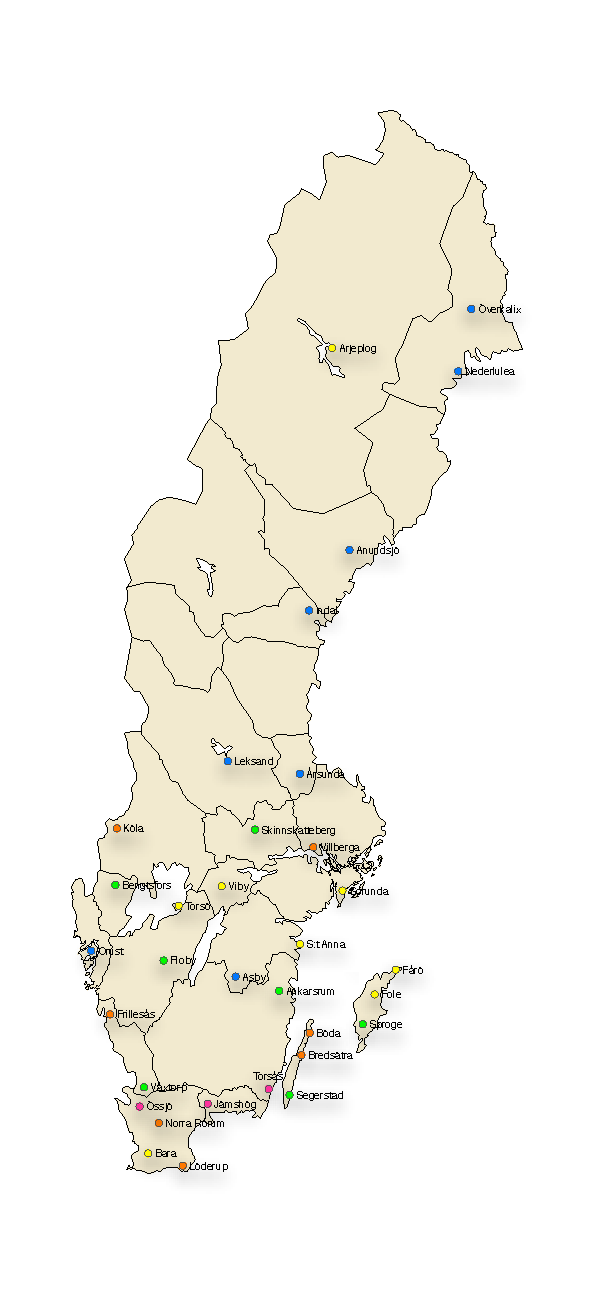
\includegraphics[width=0.32\textwidth]{Sverigekarta-Landskap-Swedia}
  \label{agree-clusters-small}
  \caption{Swedia, Clusters Common to All 3 Methods}
\end{figure}

\begin{figure}
  \includegraphics[width=0.5\textwidth]{Sverigekarta-Landskap-mds-dep}
  \label{mds-dep-small}
  \caption{Swedia, Multi-Dimensional Scaling of Dependency Path Distance}
\end{figure}

Once both dialectologic and dialectometric regions have been
identified, comparison is straightforward. Each region can be checked
for overlap---regions with a greater overlap area are better matches.

The real problem in identifying regions is that there has not been
enough dialectology work on Swedish syntax yet: numerous identified
isogloss bundles are indicative of a well understood area of
dialectology. In Swedish syntax, few regions are well-known and
well-documented enough to have isogloss bundles. It is possible that
dialectometry will lead the way in providing answers in this
area.

\subsection{Distances}

Although comparing distances from dialectometry to qualitative
research in dialectology is possible, it is unlikely to be useful in
this dissertation because of the previously mentioned lack of
developed Swedish dialectology in syntax. When it is possible,
one either looks for differences in size of isogloss bundle, or (more
weakly) statements like ``in general, Southern
Swedish is syntactically identical to Standard Swedish''
\cite{rosenkvist07} or ``there are numerous differences between
dialect X and the standard language''.

\section{Alternate Distance Measures}

% maybe re-organize to be (1),(2),(3) therefore it's simple
% instead of "it's simple", (1) (2) (3).
Of the measures considered in this dissertation, $R$ is the
simplest---it's the sum of difference in feature counts. It is almost
the simplest statistical measure possible; it uses very simple math
and treats its feature as opaque symbols.  Despite this, R appears to
perform better, or at least more consistently, than other measures
that have been tested in this dissertation. It gives significant
results across a larger variety of feature sets than more complicated
measures do.

The question of measure is more important than feature set because
measures are harder to construct than feature sets, and even harder to
combine compared to feature sets. However, the distance measures
tested so far do not have a greater effect on significance also have a
greater effect on significance.

TODO: The introduction and justification here are worthless. Their
statements are false or irrelevant. So maybe this section as a whole
is worthless.

There are basically two directions to explore when creating an
distance measure to replace $R$. The first direction is to address
$R$'s simplicity by finding a more complex measure, such as using more
sophisticated ways to measure difference or the capability to use
numeric features. The second direction is to address $R$'s ignorance
of syntax by finding a measure with specific knowledge of syntax. The
first direction is easier, given the statistical bent of the corpus
used here and the number of statistical measures commonly used in
computational linguistics. A number of these measures are described in
the Methods chapter after the description of $R$.  Additionally, the
statistical framework is powerful enough that most syntax-specific
knowledge can be represented in terms of features instead of
integrated into the distance measure's algorithm.

TODO: ``Statistical'' is not quite the right word here.

Indeed, it is so difficult to think of syntax-specific algorithms that
none are presented in this dissertation. However, a number of more
complicated statistical measures are presented and some are tested. Goebl's
Weighted Identity Value (originally, Gewichteter Identit\"atswert) is
the earliest to be used in dialectometry, but others such as
Kullback-Leibler divergence and its variants are a good fit because of
their similarity to $R$.

\subsection{Syntax-specific distance measures}

As mentioned above, syntax-specific measures are more difficult to
specify---they must somehow incorporate knowledge of syntax in the
measure itself, in such a way that cannot be reified as features that
could then be processed by a generic statistical measure. This is
difficult when working with syntactic corpora; the amount of
information about each sentence is much lower than the amount of
information about each word in a traditional dialectology corpus of
phonology. Specifically, there is no alignment between sentences, nor is
there a predefined list of sentences to be elicited. In addition,
there is no well-accepted model equivalent the one set out by
\namecite{chomsky68}, which can be further augmented by later work in
phonology, such as \quotecite{goldsmith76} autosegmental
phonology. Dialectology work on phonology has relaxed these
assumptions, but switching to statistical analysis of unordered
corpora \cite{sanders06} and \cite{hinrichs07} has not
been as successful as abandoning distinctive features \cite{heeringa04}.

The hidden structure available for syntax is the parse---whether this
is a constituent parse, dependency parse or some variant of shallow
parse. Working by analogy from phonology, segments have hidden
structure in the form of distinctive features. Segment order in
phonology corresponds to word order in syntax. Unfortunately, as just
mentioned, the analogy does not extend to corpus order. However, there
is one piece of information that is not available to phonology (at
least pre-autosegmental phonology): the upper structure is
connected. For the current set of experiments, the upper structure is
processed, divided and assigned as features attached to an individual
word in the form of leaf-ancestor paths or dependency paths. This
approach allows the features to be given to $R$ and treated as if they
are independent, which is of course not true.

However, even taking advantage of this connected upper structure only
provides additional features per sentence. These features can be
profitably added to the others when using a statistical measure, but
they do not require a new measure.

\subsection{Important note on terms}

In the preceding section, there are several terms related to distance
in use. In order from least restrictive to most restrictive, they are
`divergence', `dissimilarity' and `distance'. In this dissertation, a
`measure' is any of these three functions. A divergence is a measure
that is not required to be either symmetric or to satisfy the triangle
inequality. A dissimilarity is symmetric, but is not required to
satisfy the triangle inequality. A distance satisfies both
properties. For this dissertation, the measure only needs to be a
dissimilarity; a true distance is not needed.

All three kinds of functions must always return positive numbers, and
only return 0 for corpora that are equal.  A symmetric function
returns the same number whether measuring from point X to point Y or
from point Y to point X. The triangle inequality means that distance
from point X to point Y plus point Y to point Z is at least as long as
traveling straight from point X to point Z.  If this is true, it
means that the function is measuring the same thing between all
corpora and therefore that the shortest path between two points can be
shortened by substituting a path with fewer intermediate
points. Equations
\ref{distance-properties-positive}-\ref{distance-properties-triangle}
list the properties formally.

\begin{equation}
  d(x,y) \ge 0
  \label{distance-properties-positive}
\end{equation}

\begin{equation}
 d(x,y) = 0 \textrm{ iff } x=y
\end{equation}

\begin{equation}
  d(x,y) = d(y,x)
\end{equation}

\begin{equation}
  d(x,y) + d(y,z) \ge d(x,z)
\label{distance-properties-triangle}
\end{equation}

\section{Question 2 : Best Features}

The second question of this dissertation reflects the fact that the
overall question of syntax distance for dialectometry has two
parts. The first question deals with whether a distance measure like
$R$ can be found that works with features extracted from a
large unaligned corpus. Therefore, the second question deals with the
feature sets used as input: how to specify them, how to generate them,
and how to evaluate them.

Specification is an easier question; feature sets are easier
to create than distance measure algorithms, as the preceding
discussion of alternate distance measures has shown. In addition,
feature sets are easier to combine and to tweak. The real problem is
not in specification of feature sets, but that new feature sets must
be evaluated, since there is no accepted standard as with phonology's
distinctive features.

For example, in previous work, I showed that leaf-ancestor paths have a small
advantage of trigrams \cite{sanders07} in terms of finding significant
distances. This dissertation shows that, for some measures, dependency
paths have a further advantage of leaf-ancestor paths. Therefore,
Question 2 breaks into two smaller questions: (1) how can new feature sets
be proposed? and (2) how can they be evaluated against one another?

\subsection{Proposing Feature Sets}

New feature sets are easy to propose. All that's needed is some way to
condense or divide the information about the sentence into symbols
that can be used as input to a statistical distance
measure. Specifically, the feature sets used in this dissertation use
per-word information, word-order information, and syntactic
information. They attach some information from the constituent tree or
dependency graph to each word, dividing the information according to
the word's position in the sentence. Trigrams attach the leaves to
each word, along with the leaves to the left and right.
Leaf-ancestor paths attach vertical slices of the tree to each
word. Dependency paths attach the path to the root to each word.

Feature sets that use other information might also be useful;
convolution kernels give a single number that captures the difference
between two trees \cite{collins01}; a similar feature that captures
aspects of a single tree such as depth, branching degree or
homogeneity might be useful. Besides this, there are numerous simple
features used in other computational linguistic work that attempt to
capture the most important characteristics of a sentence in a simple,
ad-hoc way, such as the first or last $n$ words of a sentence, a
certain number of words surrounding the predicate, or sentence length.

Even before looking at results, it seems that each of these has its
own advantages and disadvantages. Simpler features like
first-$n$-words are presumably intended to reflect
processing priorities (CITE if I want to keep this in
here). Leaf-ancestor paths capture upper structure of the constituent
parse. Dependency paths capture similar information but with more
emphasis on long-distance relations between words. Trigrams capture
less detail but are less influenced by annotator error since they
require only part-of-speech annotation.

\subsection{Evaluating Feature Sets}

Because evaluation of feature set performance is necessarily evaluation
of the overall combination of feature set and measure, the previously
discussed measures of agreement with dialectology should all be used
as measures of performance. With the distance measure held constant,
the different feature sets can be evaluated against one another.

In addition to comparison against dialectology, a couple of additional
measures indicate feature set quality. Of the two, geographical
distance is more important; although there is no {\it a priori} reason
for geographical distance to match dialect distance, the dialectology
literature overwhelmingly shows that it does \cite{gooskens04a} (and
probably \cite{heeringa04}, \cite{kondrak02}, and others).

% rewrite to avoid overuse of important.
Statistical significance is also important. Although significance does not
necessarily indicate a good set of features, a lack of statistical
significance indicates that the feature set does not allow the distance
measure to find valid distances.

\section{Question 3 : Agreement with Phonological Dialectometry}

Finally, agreement with phonological dialectometry is a useful
indicator of quality. Agreement with phonology indicates a good
feature set, but cannot indicate a bad feature set. Phonological
boundaries need not agree with syntactic boundaries, but it seems very
likely that they do. This is the reverse of statistical significance's
import for syntax distance---it can only indicate a bad feature set
and can never prove a good feature set.

There is very little phonological dialectometry for Swedish, so this
comparison may not be valid yet. The only published paper, to my knowledge, is
\namecite{leinonen08}, as well as Leinonen's as-yet-unpublished dissertation
(2010).


%%% Local Variables: 
%%% mode: latex
%%% TeX-master: "dissertation.tex"
%%% End: 
